\documentclass[conference]{IEEEtran}
% Compilar com PDFLaTeX, BibTeX, PDFLaTeX, PDFLaTeX.
\usepackage[utf8]{inputenc}
\usepackage[T1]{fontenc}
\usepackage[brazil]{babel}
\usepackage{lmodern}
\usepackage{cite}
\usepackage{amsmath,amssymb}
\usepackage{graphicx}
\graphicspath{{figuras/}}
\usepackage{booktabs,tabularx,array}
\usepackage{float} % Somente para manter a tabela de rastreabilidade junto ao apêndice
\usepackage{xurl}
\usepackage[hidelinks]{hyperref}
\usepackage{microtype}
\usepackage{balance}
\newcolumntype{Y}{>{\raggedright\arraybackslash}X}
\begin{document}
\title{Monitoramento de condições em compressores ferroviários por ciclos de pressurização e telemetria IoT simulada: estudo retrospectivo com o MetroPT-3}
\author{%
\IEEEauthorblockN{Jorge Luca de Azevedo dos Reis}
\IEEEauthorblockA{Programa de Pós-Graduação em Engenharia Elétrica (PPGEE)\\
Universidade Federal do Acre (UFAC)\\
Rio Branco, Brasil\\
jorge.reis@sou.ufac.br}
% IMPORTANTE: incluir outro autor apenas com autorização/autoria confirmadas.
% \and
% \IEEEauthorblockN{José Humberto Araújo Monteiro}
% \IEEEauthorblockA{Universidade Federal do Acre (UFAC)\\Rio Branco, Brasil}
}
\maketitle


\begin{abstract}
O monitoramento de condições de unidades pneumáticas ferroviárias exige distinguir ciclos operacionais atípicos de evidências verificadas de defeito. Este artigo apresenta a revisão metodológica e a avaliação retrospectiva de um detector interpretável de recuperação lenta de pressão, associado a um protótipo de telemetria IoT simulada. Empregou-se o arquivo público MetroPT-3 com 1.516.948 registros de sensores, separados predominantemente por aproximadamente dez segundos. Foram identificadas 15.769 fases sob carga; 10.417 atenderam aos critérios de elegibilidade retrospectiva. A regra principal (R1) sinaliza uma fase iniciada entre 7,7 e 8,5 bar quando TP3 ainda não atingiu 9,7 bar após o percentil 99 do tempo de recuperação calibrado em maio (188 s). Entre 23/05 e 01/09/2020, R1 gerou 33 alertas, dos quais 13 foram emitidos nas duas horas anteriores aos horários registrados de três eventos e 20 fora das proximidades documentadas. A regra temporal de comparação com o mesmo limiar gerou 136 alertas. Em análise adicional exploratória, o uso dos percentis P95, P97,5 e P99 resultou em 363, 109 e 33 alertas totais, evidenciando o compromisso entre limiar e frequência de avisos. O processamento incremental por HTTP, SQLite e painel web reproduziu integralmente os 190 alertas das três regras originais. Os resultados demonstram viabilidade computacional e maior seletividade relativa da regra condicionada à pressão; não comprovam previsão prospectiva de vazamentos, devido à rotulagem parcial, ao número reduzido de eventos e à seleção exploratória das hipóteses.
\end{abstract}

\begin{IEEEkeywords}
manutenção baseada em condição; Internet Industrial das Coisas; compressor ferroviário; ciclos de pressurização; detecção de anomalias; MetroPT-3.
\end{IEEEkeywords}

\section*{Abstract}
Condition monitoring of railway pneumatic units requires distinguishing atypical operating cycles from verified equipment faults. This paper presents a methodological revision and a retrospective assessment of an interpretable slow-pressure-recovery detector linked to a simulated IoT telemetry prototype. The public MetroPT-3 file comprises 1,516,948 sensor readings, predominantly separated by approximately ten seconds. A total of 15,769 loaded-operation phases were identified; 10,417 met retrospective eligibility criteria. The primary rule (R1) raises an alert when a phase starting between 7.7 and 8.5 bar fails to reach 9.7 bar in TP3 after the 99th percentile of calibration recovery times (188 s). Between 23 May and 1 September 2020, R1 generated 33 alerts, including 13 within the two hours preceding three documented event timestamps and 20 outside the predefined event vicinities. A time-only comparator at the same threshold generated 136 alerts. An additional exploratory sensitivity analysis yielded 363, 109, and 33 total alerts at the 95th, 97.5th, and 99th percentiles, respectively. Incremental HTTP-based processing, SQLite storage, and a web dashboard reproduced all 190 original alerts across the three rules. These findings support computational feasibility and the relatively higher selectivity of pressure-conditioned alerts, but do not establish prospective air-leak prediction performance because annotations are incomplete, the event count is small, and hypotheses were developed exploratorily.
\par\noindent\textbf{Keywords:} condition-based maintenance; Industrial Internet of Things; railway compressor; pressurization cycles; anomaly detection; MetroPT-3.

\section{Introdução}

A instrumentação de ativos industriais permite acompanhar pressões, correntes, temperaturas e sinais discretos em séries temporais, mas a conversão dessas medições em ações de manutenção depende da compreensão do processo e de critérios capazes de distinguir flutuações de demanda de degradação do equipamento. A Internet das Coisas (IoT) integra aquisição, comunicação e processamento; entretanto, dispor de uma cadeia de telemetria não implica comprovar diagnóstico ou prognóstico \cite{atzori2010survey,lee2015cps}.

Em uma unidade de produção de ar (Air Production Unit -- APU) ferroviária, o compressor atende cargas pneumáticas de consumo variável. A pressão resultante depende da capacidade de suprimento, do consumo e de possíveis perdas, de modo que fases longas de acionamento não correspondem, necessariamente, a vazamentos. O MetroPT-3 constitui uma oportunidade de investigar essas ambiguidades a partir de observações reais e registros de manutenção associados \cite{davari2021metropt3,veloso2022metropt}.

Este estudo busca responder: em uma avaliação retrospectiva, o tempo de recuperação da pressão durante fases sob carga permite gerar avisos anteriores aos horários documentados de eventos de falha e pode ser processado incrementalmente em uma arquitetura computacional de telemetria? O termo ``anterior'' refere-se estritamente ao horário da anotação administrativa, sem garantia de que a manifestação física do defeito ainda não havia começado.

As contribuições são: (i) auditoria da versão concreta do CSV; (ii) descrição de um detector de primeira passagem de pressão com manejo de interrupções de telemetria; (iii) comparação com dois critérios temporais sob a mesma condição inicial; (iv) análise descritiva e de sensibilidade exploratória; (v) integração funcional de replay por HTTP, armazenamento SQLite e visualização; e (vi) delimitação explícita das afirmações sustentadas por apenas três eventos avaliados.

\section{Fundamentação teórica}

\subsection{Monitoramento de condições, diagnóstico e prognóstico}

Monitoramento baseado em condição consiste em coletar e interpretar sinais relacionados ao desempenho de máquinas para apoiar decisões de manutenção. A norma ISO 17359:2018~\cite{iso17359} apresenta diretrizes gerais para a organização de programas dessa natureza, mas não estabelece os limiares específicos usados neste experimento. Jardine, Lin e Banjevic~\cite{jardine2006review} distinguem procedimentos de diagnóstico de condição atual e de prognóstico de eventos futuros. Dessa forma, um alerta tecnicamente verificável de recuperação lenta não é automaticamente uma previsão de vazamento.

É igualmente necessário distinguir um período ``sem evento documentado'' de um período certificado como saudável. Na ausência de inspeção exaustiva, sinais fora dos intervalos registrados não podem receber, sem ressalvas, o rótulo de falsos positivos. Esse princípio é coerente com a detecção contextual de anomalias, na qual observações aparentemente raras podem expressar regimes legítimos de trabalho \cite{chandola2009anomaly}.

\subsection{Princípios físicos da pressurização de uma APU}

Em termos qualitativos, a evolução da pressão de um reservatório conectado a um compressor depende do fluxo efetivo fornecido, do consumo pneumático e das perdas. Uma relação conceitual de balanço pode ser escrita como

\begin{equation}\label{eq:balanco}\frac{dP}{dt}\approx K(t)\bigl[Q_{\mathrm{comp}}(t)-Q_{\mathrm{cons}}(t)-Q_{\mathrm{perdas}}(t)\bigr].\end{equation}

Em que $K(t)$ representa fatores agregados de compressibilidade e volume efetivo. Esta expressão é uma idealização ilustrativa, não um modelo identificado ou validado para o MetroPT-3, e não foi utilizada para estimar vazão, volume ou tamanho de vazamento.

A pressão TP3 é medida no painel pneumático; a corrente do motor e o estado DV\_eletric ajudam a caracterizar a operação sob carga. Uma recuperação lenta pode resultar de diminuição da capacidade de pressurização, vazamento, consumo elevado dos sistemas atendidos ou transições de operação. Como o consumo exato dos usuários pneumáticos não é conhecido neste recorte, a causa de um episódio lento não é identificável exclusivamente a partir do indicador de tempo. Os estudos sobre o próprio sistema MetroPT detalham a instrumentação e ilustram diferentes falhas operacionais (BARROS et al., 2020; VELOSO et al., 2022).

\subsection{Arquitetura IIoT e limites de demonstrações com replay}

Uma arquitetura IoT industrial pode envolver sensores, aquisição embarcada, rede, persistência de dados, análise contínua e interface de supervisão. A literatura sobre sistemas ciberfísicos enfatiza o encadeamento das funções físicas e informacionais \cite{lee2015cps}. No presente estudo foram implementadas apenas as etapas computacionais: o histórico de sensores foi transmitido cronologicamente por HTTP dentro do mesmo computador, sem sensores físicos, transporte embarcado, MQTT, nuvem ou testes de disponibilidade e segurança de redes industriais.

\subsection{Trabalhos relacionados e posicionamento do estudo}

Davari et al.~\cite{davari2021predictive} e Barros et al.~\cite{barros2020failure} investigaram anomalias e falhas de APU em ambiente ferroviário; Veloso et al.~\cite{veloso2022metropt} descreveram o conjunto de dados e sua validação; García-Méndez et al.~\cite{garciamendez2025explainable} propuseram uma estrutura explicável de aprendizado de máquina em fluxo. A literatura demonstra a relevância de cenários com sensores heterogêneos, mas os conjuntos de rótulos, versões de dados e objetivos diferem. Não seria metodologicamente correto comparar diretamente o número de alertas deste estudo com taxas reportadas nesses trabalhos.

\begin{table*}[!t]
\centering
\footnotesize
\setlength{\tabcolsep}{4pt}
\renewcommand{\arraystretch}{1.15}
\caption{Trabalhos relacionados e diferenças frente ao presente estudo.}
\label{tab:0}
\begin{tabularx}{\textwidth}{@{}p{0.20\textwidth}p{0.32\textwidth}X@{}}
\toprule
\textbf{Referência} & \textbf{Foco e material analisado} & \textbf{Distinção frente a este estudo} \\
\midrule
Barros et al.~\cite{barros2020failure} & Detecção de falhas de APU em contexto operacional & Enfoque em detecção de falhas; não reproduzido neste protocolo. \\
Davari et al.~\cite{davari2021predictive} & Detecção de anomalias por aprendizado profundo na APU & Modelos e rótulos não diretamente comparados ao limiar físico. \\
Veloso et al.~\cite{veloso2022metropt} & Descrição e validação técnica do MetroPT & Fonte de contexto e instrumentação; versões exigem distinção. \\
García-Méndez et al.~\cite{garciamendez2025explainable} & Fluxo de aprendizado de máquina com explicabilidade & Abordagem supervisionada; rótulos e amostragens distintos. \\
Presente trabalho & Primeira passagem de TP3 + replay HTTP local & Ênfase em interpretabilidade, rastreabilidade e equivalência de execução. \\
\bottomrule
\end{tabularx}
\end{table*}

\section{Materiais e métodos}

\subsection{Tipo de estudo, base e proveniência}

O desenho é aplicado, quantitativo, retrospectivo e exploratório, com prototipação computacional. A análise incidiu especificamente sobre MetroPT3(AirCompressor).csv, disponibilizado no repositório UCI sob DOI 10.24432/C5VW3R. O arquivo utilizado apresentou 1.516.948 linhas, 15 sinais industriais, uma coluna de índice e timestamp, observações entre 01/02/2020 e 01/09/2020, sem valores faltantes ou timestamps duplicados. O SHA-256 do CSV efetivamente analisado é \nolinkurl{db30ccb4ea402e3c8bf2c99db06e288d4f2a772f6928f9dbe26a920d69793e24}~\cite{davari2021metropt3}

Embora a descrição histórica de aquisição mencione 1 Hz, a versão do arquivo aqui processada possui diferenças entre timestamps predominantemente próximas de dez segundos (aproximadamente 0,1 Hz em trechos típicos), além de 331 lacunas superiores a 60 segundos, incluindo 160 acima de uma hora. A base UCI disponibilizada possui 1.516.948 registros; dados de outra edição da família MetroPT descritos na literatura não foram concatenados. Não houve interpolação de longos períodos ausentes \cite{davari2021metropt3,veloso2022metropt}

Os sinais empregados diretamente na regra principal foram TP3 (pressão em bar), Motor\_current (A) e DV\_eletric (sinal de controle). Oil\_temperature e as demais variáveis foram usadas apenas nas etapas exploratórias anteriores. Não se estabeleceu medição direta de vazão perdida ou da demanda pneumática de cada consumidor.

\begin{table}[!t]
\centering
\caption{Eventos documentados no MetroPT-3.}
\label{tab:1}
\footnotesize
\setlength{\tabcolsep}{3.5pt}
\renewcommand{\arraystretch}{1.12}
\begin{tabular}{@{}c c c@{}}
\toprule
\textbf{Evento} & \textbf{Início documentado} & \textbf{Fim documentado} \\
\midrule
F1 & \shortstack{18/04/2020\\00:00} & \shortstack{18/04/2020\\23:59} \\
F2 & \shortstack{29/05/2020\\23:30} & \shortstack{30/05/2020\\06:00} \\
F3 & \shortstack{05/06/2020\\10:00} & \shortstack{07/06/2020\\14:30} \\
F4 & \shortstack{15/07/2020\\14:30} & \shortstack{15/07/2020\\19:00} \\
\bottomrule
\end{tabular}
\vspace{2pt}
\parbox{\columnwidth}{\raggedright\scriptsize\textit{Nota:} F1 foi inspecionado na fase exploratória e não integrou o teste final; F2, F3 e F4 compõem a avaliação retrospectiva.}
\end{table}

\subsection{Segmentação em fases sob carga e cobertura temporal}

Foi adotada a definição operacional exploratória de carga:

\begin{equation}\label{eq:estado}L(t)=\begin{cases}1,&I_{\mathrm{motor}}(t)>2\ \mathrm{A}\ \mathrm{e}\ DV_{\mathrm{eletric}}(t)>0{,}5;\\0,&\text{caso contrário.}\end{cases}\end{equation}

Uma fase sob carga começa na transição observada para L=1 e termina na transição para L=0 ou quando o intervalo entre registros excede 30 s. Esta regra impede considerar telemetria ausente como tempo comprovadamente observado. O critério não corresponde a uma especificação de fabricante ou validação independente do estado mecânico.

Para estatísticas retrospectivas de ciclos completos, exigiram-se transições observadas nas duas extremidades, pressão inicial TP3 entre 7,7 e 8,5 bar e duração de pelo menos 35 s. Identificaram-se 15.769 fases sob carga e 10.417 ciclos completos elegíveis. Diferentemente dessa seleção retrospectiva, a emissão de avisos em fluxo usa somente a condição observável no início da fase e os valores que chegam posteriormente, sem examinar o fim da fase para autorizar um alerta.

\subsection{Variável de tempo até a pressão-alvo e censura}

Para uma fase $i$ iniciada em $t_{0,i}$ e terminada em $t_{e,i}$, definiu-se o tempo da primeira recuperação de pressão como:

\begin{equation}\label{eq:recuperacao}\begin{aligned}T_{9{,}7,i}=\min\bigl\{&t-t_{0,i}:t\in[t_{0,i},t_{e,i}],\\&L(t)=1,\ \mathrm{TP3}(t)\geq 9{,}7\ \mathrm{bar}\bigr\}.\end{aligned}\end{equation}

Se a fase termina, sofre uma lacuna superior a 30 s ou chega ao fim do arquivo sem alcançar a referência, o tempo de primeira recuperação permanece não observado (censurado no limite do acompanhamento). Ausência de recuperação não equivale a tempo de recuperação igual a zero.

O alvo TP3=9,7 bar e a faixa de partida 7,7--8,5 bar são escolhas analíticas exploratórias resultantes da inspeção do histórico. Como também foram analisados eventos que viriam a compor o conjunto de avaliação, essas escolhas não atendem aos requisitos de avaliação cega. O limiar foi mantido na análise de sensibilidade para evitar alterar múltiplas dimensões simultaneamente.

\subsection{Calibração e definição das três regras}

Usou-se 01/05/2020--22/05/2020 para a calibração estatística e 23/05/2020--01/09/2020 para a avaliação retrospectiva. Na calibração, 953 ciclos eram elegíveis; 948 atingiram a pressão-alvo e cinco não a atingiram. O percentil 99 da primeira recuperação entre os 948 ciclos observados resultou em 188 s; o percentil 99 da duração de todos os 953 ciclos completos resultou em 337,12 s. Como os cinco tempos censurados não entraram no cálculo do P99 de recuperação, a distribuição de cauda pode estar subestimada.

As três regras compartilham as condições de estar sob carga e de começar a fase com TP3 entre 7,7 e 8,5 bar. R1 -- recuperação lenta: emitir um alerta quando a fase alcança pelo menos 188 s e ainda não houve leitura TP3 $\geq 9{,}7$ bar. R2 -- carga prolongada: emitir um alerta quando a fase alcança 337,12 s, independentemente de a pressão-alvo já ter sido alcançada. R3 -- comparação somente temporal: emitir um alerta aos 188 s, também independentemente da recuperação. Cada regra emite no máximo um alerta por fase. O instante efetivo é o primeiro timestamp de leitura que satisfaz o limiar temporal, não um instante artificial interpolado.

Essa redação elimina a ambiguidade da versão anterior: ``independentemente da pressão'' em R2 e R3 significa independentemente da pressão ao longo da recuperação, mas não da mesma pressão inicial usada para elegibilidade. R1 $\times$ R3 isola, portanto, a exigência adicional de pressão ainda não recuperada no instante do aviso.

\subsection{Critérios de avaliação retrospectiva}

Para cada evento com início reportado tf, contou-se a existência e o número de alertas no intervalo [tf-2 h, tf). Para contabilizar avisos fora das proximidades dos eventos conhecidos, removeram-se [tf-2 h, término\_reportado+24 h] para F2--F4. Alertas ocorridos nas 24 horas posteriores foram apresentados separadamente para que as categorias totalizem corretamente. A janela de duas horas foi escolhida no processo exploratório e não representa antecedência ótima previamente comprovada.

Os alertas fora das proximidades não são falsos positivos confirmados. Por não existir uma rotulagem exaustiva de normalidade, não foram calculados precisão, especificidade, recall, F1, AUC ou taxa verdadeira de falsos alarmes. A razão por 30 dias expressa contagem bruta calendarizada no período de avaliação, sem correção para disponibilidade efetiva por máquina-hora.

\subsection{Análise complementar de sensibilidade (nova na versão 2)}

Para investigar a influência isolada do limiar temporal, mantiveram-se estado sob carga, pressão de partida, alvo de 9,7 bar, recorte de calibração e divisão cronológica. Reexecutou-se R1 com os percentis P95, P97,5 e P99 dos tempos observados de recuperação no período de calibração, sem ajustar esses valores a partir dos rótulos de F2--F4. A análise foi planejada após conhecimento dos eventos, portanto é uma análise pós-hoc descritiva, e não uma validação externa. Os alertas foram emitidos sobre os timestamps reais do CSV por meio do mesmo extrator e função de alerta utilizados na Etapa 4.

\subsection{Reprodutibilidade e arquitetura de replay}

A extração das fases, o cálculo dos limiares e os registros foram preservados em código Python e arquivos CSV/JSON. O detector incremental recebe leituras cronológicas por POST HTTP em ambiente local, persiste dados e alertas em SQLite e expõe indicadores ao painel. Os testes cortaram o histórico antes dos eventos para verificar que decisões passadas não mudavam com novas amostras. A equivalência de implementação foi aferida comparando pares exatos (nome da regra, timestamp de alerta) entre execução incremental e processamento retrospectivo.

\begin{figure*}[!t]
\centering
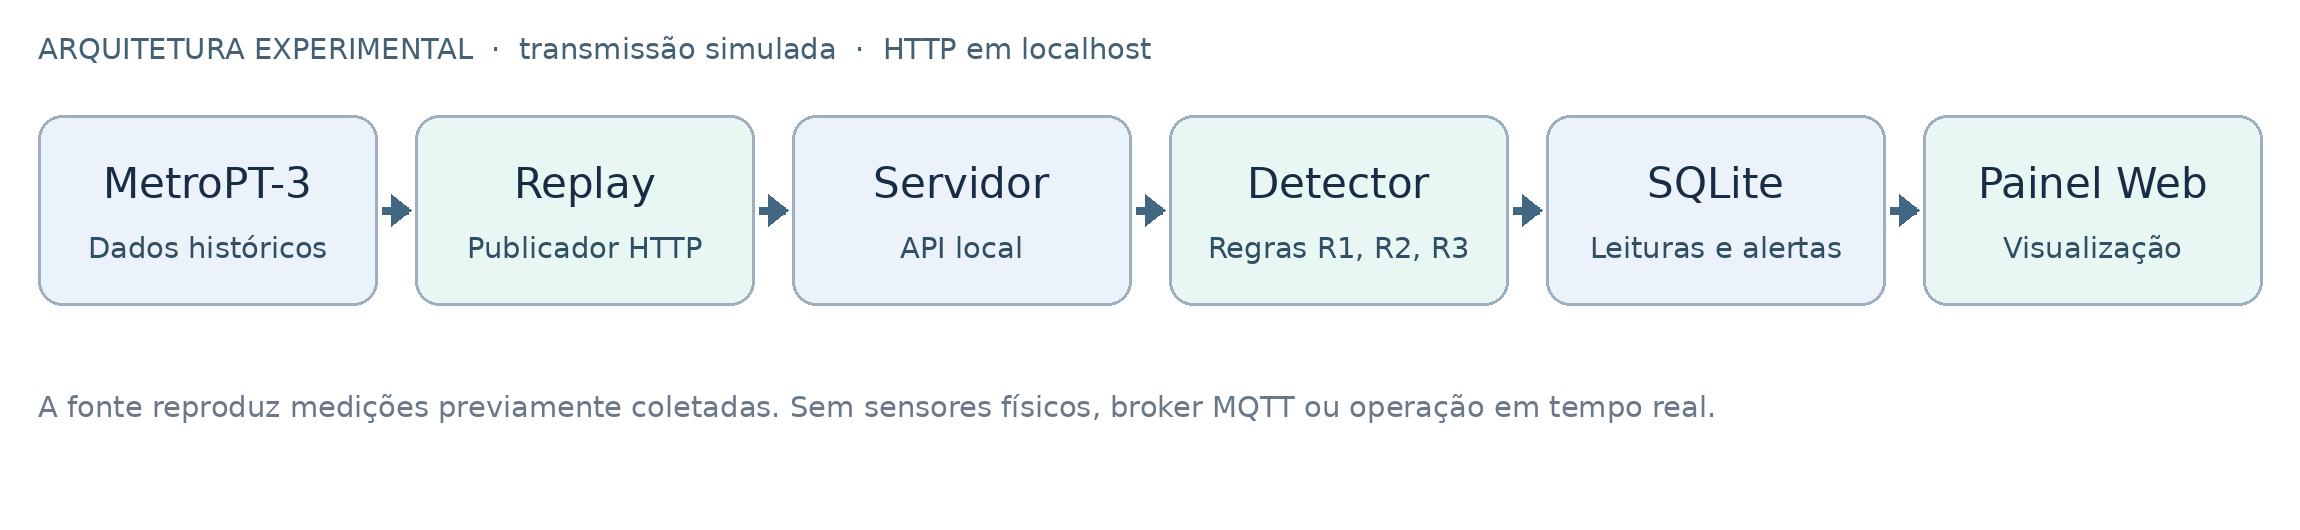
\includegraphics[width=\textwidth]{01_arquitetura_iot.png}
\caption{Arquitetura lógica do protótipo de reprodução de telemetria histórica. Comunicação HTTP local; não houve instalação física de IoT.}
\label{fig:arquitetura}
\end{figure*}

\section{Resultados}

\subsection{Caracterização da operação e do comportamento pré-evento}

Os 10.417 ciclos completos elegíveis apresentaram duração mediana de aproximadamente 129 s e aumento mediano de TP3 de aproximadamente 2,02 bar. Nas duas horas anteriores a F2 e F3, os ciclos concluídos alcançaram 9,7 bar em mediana próxima de 99 s, semelhante ao comportamento central da calibração. Já antes de F4, doze ciclos concluídos apresentaram mediana de recuperação de 218 s, o que sugere mudança na dinâmica operacional, mas não identifica isoladamente o mecanismo causal.

\begin{figure}[!t]
\centering
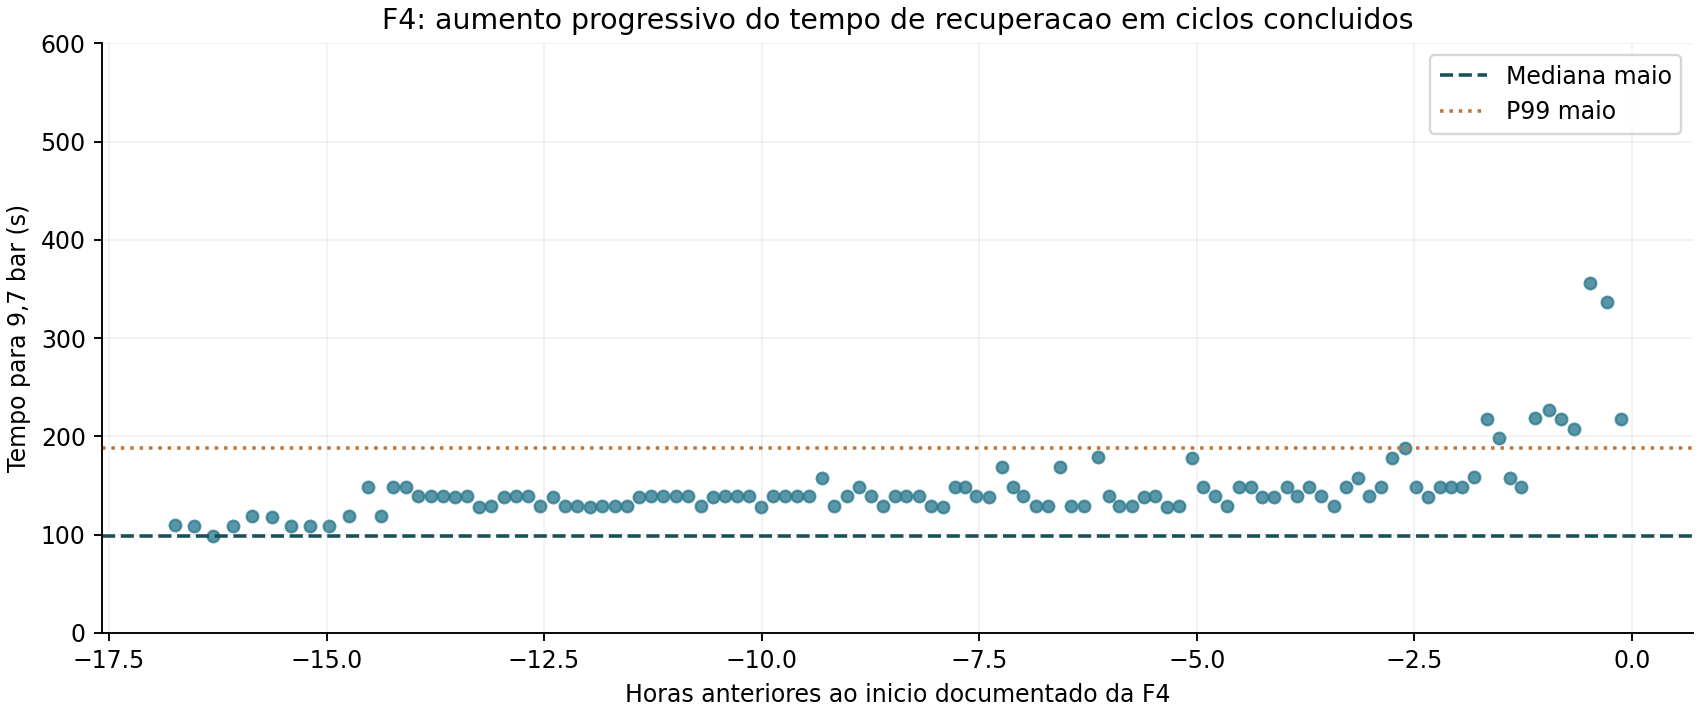
\includegraphics[width=\columnwidth]{02_recuperacao_f4.png}
\caption{Tempos de primeira recuperação de pressão nos ciclos anteriores ao início documentado do evento F4.}
\label{fig:recuperacao_f4}
\end{figure}

\subsection{Contagem de alertas e categorias mutuamente excludentes}

\begin{table}[!t]
\centering
\caption{Distribuição mutuamente excludente dos alertas no teste.}
\label{tab:2}
\footnotesize
\setlength{\tabcolsep}{4pt}
\renewcommand{\arraystretch}{1.13}
\begin{tabularx}{\columnwidth}{@{}Y r r r@{}}
\toprule
\textbf{Indicador} & \textbf{R1} & \textbf{R2} & \textbf{R3} \\
\midrule
Total de alertas & 33 & 21 & 136 \\
Nas 2 h anteriores & 13 & 7 & 18 \\
Durante as falhas & 0 & 1 & 0 \\
Até 24 h após & 0 & 0 & 3 \\
Fora das proximidades & 20 & 13 & 115 \\
Eventos com aviso prévio & 3/3 & 3/3 & 3/3 \\
\bottomrule
\end{tabularx}
\vspace{2pt}
\parbox{\columnwidth}{\raggedright\scriptsize\textit{Nota:} R1: recuperação lenta; R2: carga prolongada; R3: somente tempo (188 s). As categorias temporais não se sobrepõem. ``Fora'' não significa falso positivo confirmado.}
\end{table}

R1 registrou 33 avisos, R2 registrou 21 e R3 registrou 136. A diferença R1 $\times$ R3 corresponde à exigência adicional de não ter alcançado a pressão de referência ao atingir o mesmo limite temporal: os alertas totais foram 33 e 136, respectivamente, enquanto os alertas fora das proximidades conhecidas foram 20 e 115. Isso demonstra maior seletividade da condição de pressão; não demonstra superioridade diagnóstica, pois todos os três critérios apresentaram avisos nas janelas anteriores aos mesmos três eventos documentados.

\subsection{Antecedência em relação ao registro e análise qualitativa das fases}

\begin{table}[!t]
\centering
\caption{Primeiros alertas R1 antes dos eventos documentados.}
\label{tab:3}
\footnotesize
\setlength{\tabcolsep}{3pt}
\renewcommand{\arraystretch}{1.15}
\begin{tabular}{@{}c c c r@{}}
\toprule
\textbf{Evento} & \textbf{Início reportado} & \textbf{Primeiro aviso R1} & \textbf{Min.} \\
\midrule
F2 & \shortstack{29/05/2020\\23:30:00} & \shortstack{29/05/2020\\22:51:38} & 38,37 \\
F3 & \shortstack{05/06/2020\\10:00:00} & \shortstack{05/06/2020\\09:51:38} & 8,37 \\
F4 & \shortstack{15/07/2020\\14:30:00} & \shortstack{15/07/2020\\12:48:25} & 101,58 \\
\bottomrule
\end{tabular}
\vspace{2pt}
\parbox{\columnwidth}{\raggedright\scriptsize\textit{Nota:} Houve 2, 1 e 10 avisos R1 nas duas horas anteriores, respectivamente, a F2, F3 e F4. A antecedência refere-se ao registro de manutenção.}
\end{table}

Em F2, o primeiro aviso ocorreu às 22h51min38s, com TP3=9,588 bar; a fase correspondente atingiu 9,7 bar aos 218 s e terminou às 22h52min27s, antes do início documentado às 23h30. Em F4, o primeiro aviso ocorreu às 12h48min25s, com TP3=9,364 bar; a recuperação também ocorreu aos 218 s, e a fase terminou às 12h50min04s, antes do registro das 14h30. Ambos exemplificam episódios lentos que posteriormente se normalizaram, de modo que sua ligação causal com as falhas futuras permanece indeterminada.

Em F3, a fase começou às 09h48min30s e o primeiro aviso foi emitido às 09h51min38s, com TP3=9,082 bar. A fase observada persistiu por um período prolongado sem registro de alcance da meta de 9,7 bar antes de uma interrupção do estado observado. Essa observação é mais compatível com pressurização persistentemente comprometida, mas, sem informações independentes de consumo pneumático e inspeção, também não permite atribuir o comportamento exclusivamente a vazamento. Dos 33 episódios alertados por R1 ao longo do teste, 28 atingiram a meta posteriormente.

\begin{figure*}[!t]
\centering
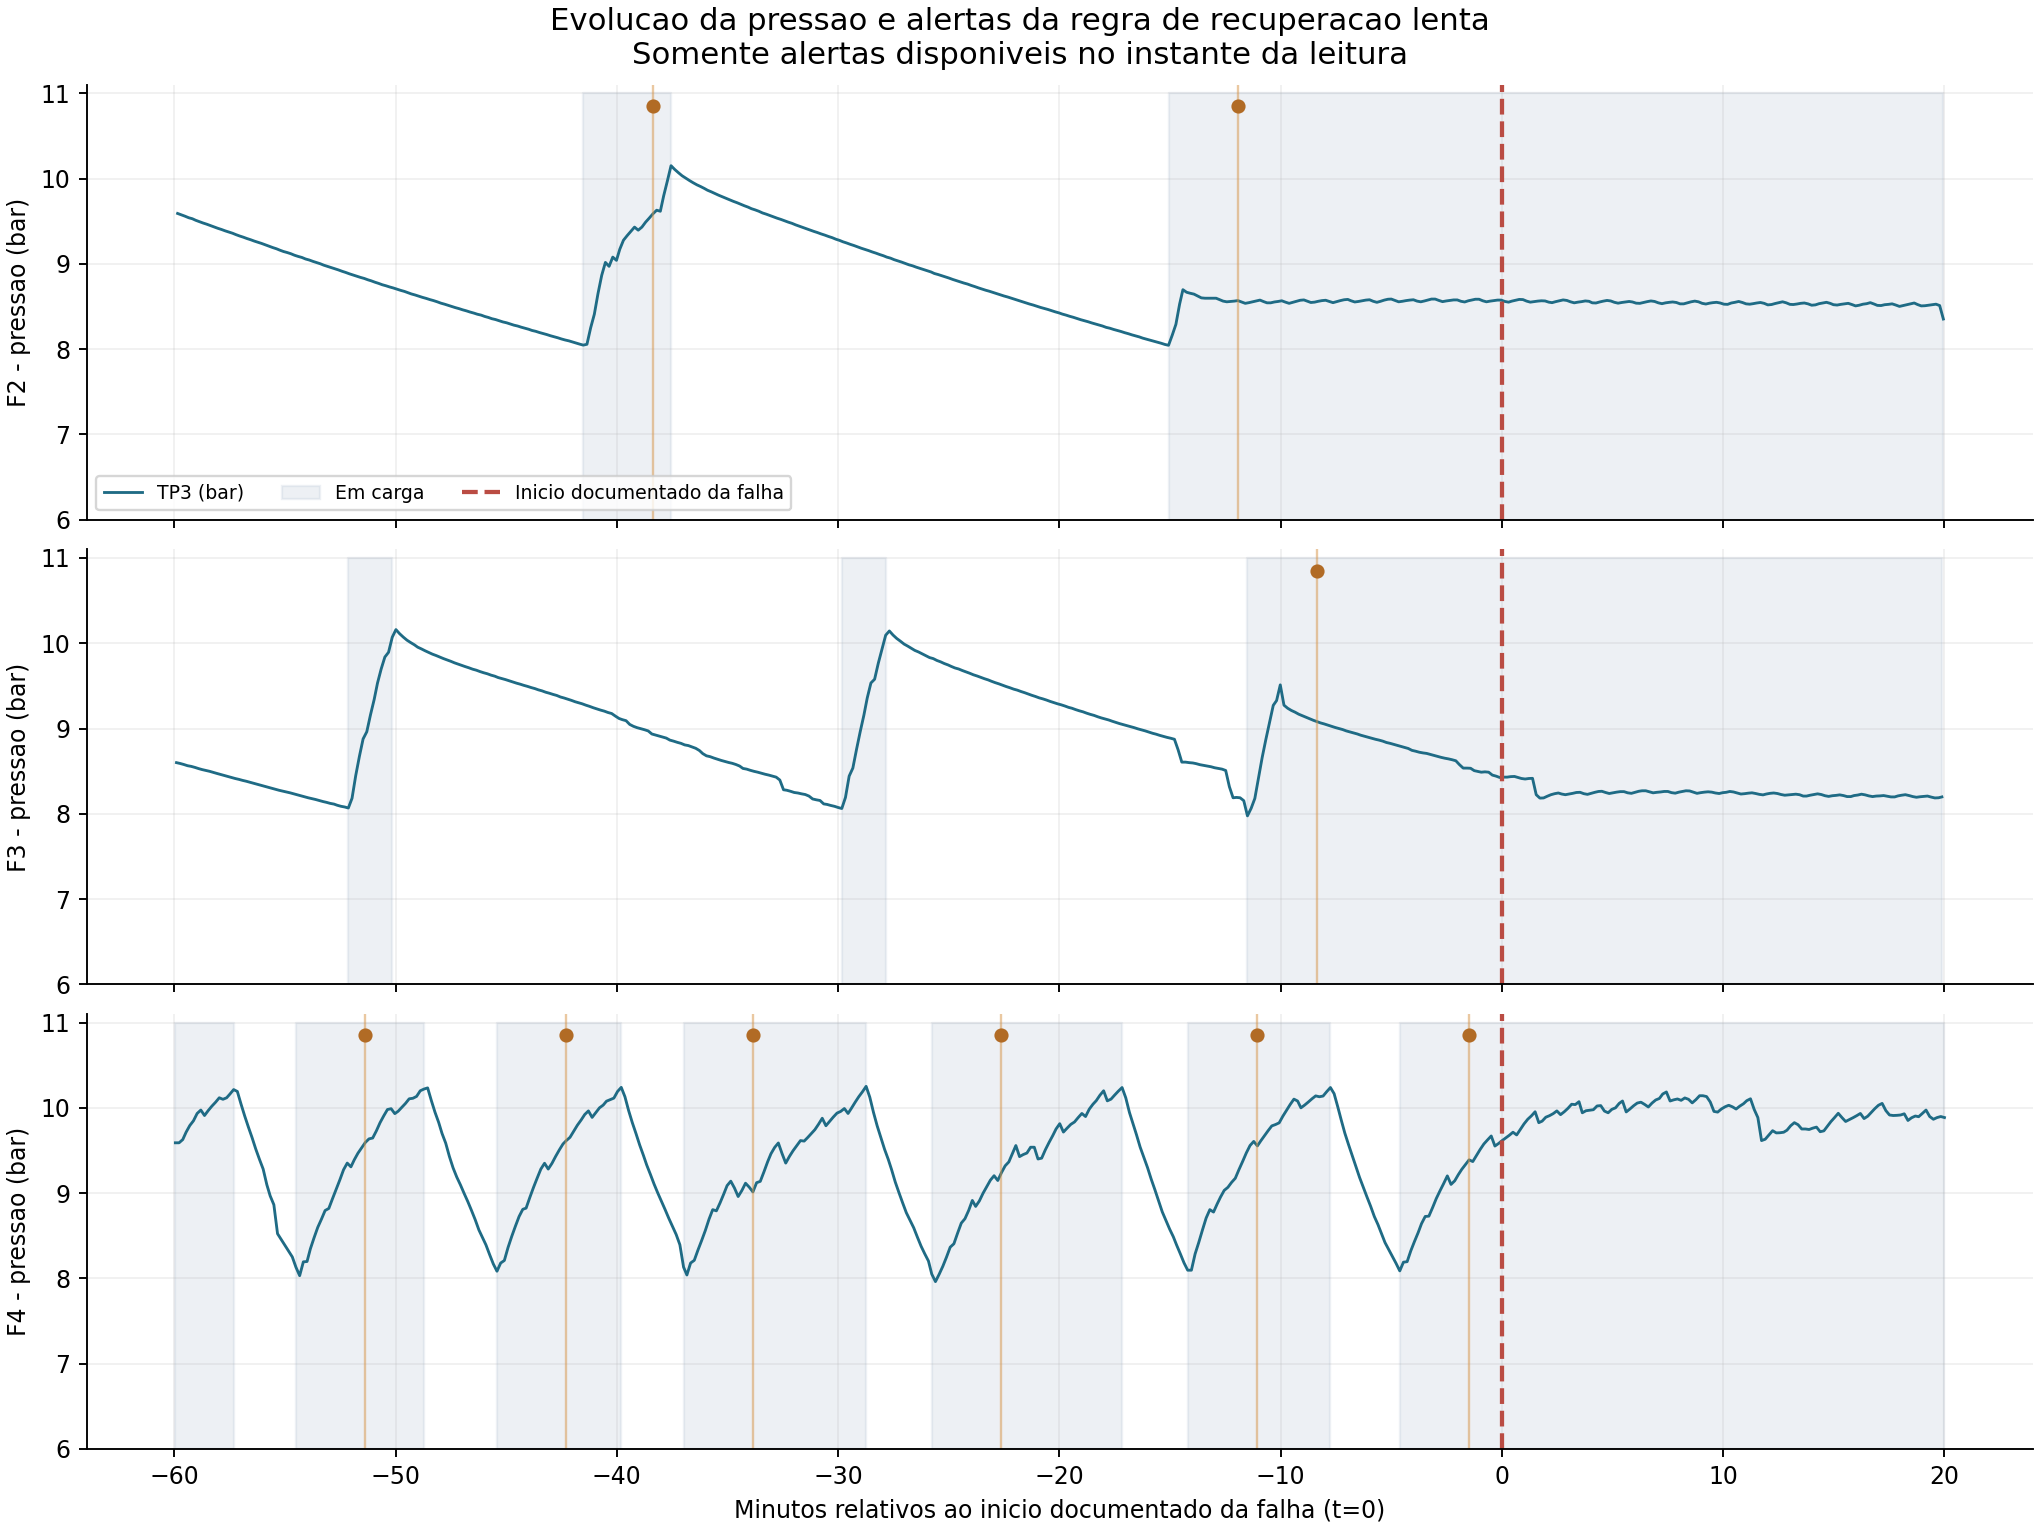
\includegraphics[width=\textwidth]{03_timeline_falhas_alertas.png}
\caption{Pressão TP3, fases sob carga e alertas de R1 nas proximidades dos registros de F2, F3 e F4.}
\label{fig:timeline}
\end{figure*}

\subsection{Sensibilidade dos alertas ao percentil de recuperação}

\begin{table}[!t]
\centering
\caption{Sensibilidade exploratória pós-hoc ao percentil.}
\label{tab:4}
\footnotesize
\setlength{\tabcolsep}{3pt}
\renewcommand{\arraystretch}{1.15}
\begin{tabularx}{\columnwidth}{@{}l r r r r r@{}}
\toprule
\textbf{Perc.} & \textbf{s} & \textbf{Total} & \textbf{Pré-2h} & \textbf{Fora} & \textbf{Eventos} \\
\midrule
P95 & 119 & 363 & 17 & 333 & 3/3 \\
P97,5 & 139 & 109 & 16 & 90 & 3/3 \\
P99 & 188 & 33 & 13 & 20 & 3/3 \\
\bottomrule
\end{tabularx}
\vspace{2pt}
\parbox{\columnwidth}{\raggedright\scriptsize\textit{Nota:} ``s'' indica limiar em segundos; ``Pré-2h'', alertas nas duas horas anteriores aos registros; ``Fora'', alertas fora das proximidades conhecidas.}
\end{table}

Ao reduzir o limite P99 de 188 s para P97,5 (139 s) e P95 (119 s), os alertas totais passaram de 33 para 109 e 363, enquanto avisos fora das proximidades passaram de 20 para 90 e 333. A presença de ao menos um alerta no horizonte de duas horas dos três eventos permaneceu igual (3/3), mas isso não representa invariância de precisão ou robustez prospectiva. Os resultados reforçam que o percentil é um parâmetro operacional com forte impacto na carga de investigação humana.

\begin{figure}[!t]
\centering
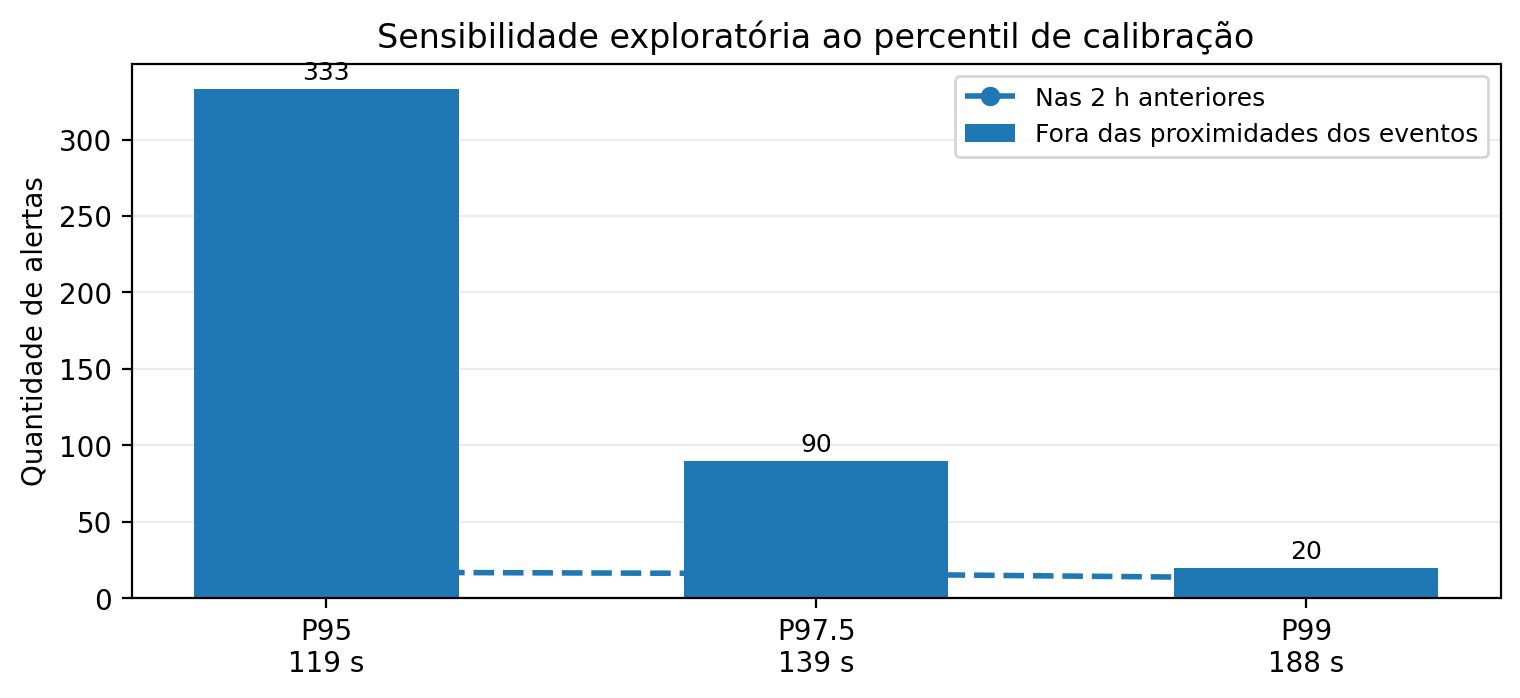
\includegraphics[width=\columnwidth]{04_sensibilidade_percentil.png}
\caption{Sensibilidade exploratória da quantidade de alertas ao percentil do tempo de recuperação; análise pós-hoc.}
\label{fig:sensibilidade}
\end{figure}

\subsection{Fidelidade de software e demonstração HTTP}

O detector incremental reproduziu, par a par e com os mesmos timestamps, os 33 alertas de R1, 21 de R2 e 136 de R3 (190 correspondências), sem diferenças frente à saída retrospectiva. Em um teste HTTP de ponta a ponta com 303 leituras históricas do recorte de F3, houve persistência dos dados e emissão de três alertas -- um por critério. A confirmação atesta consistência da implementação, e não constitui estimativa de acurácia de diagnóstico ou de latência em infraestrutura ferroviária.

\begin{figure}[!t]
\centering
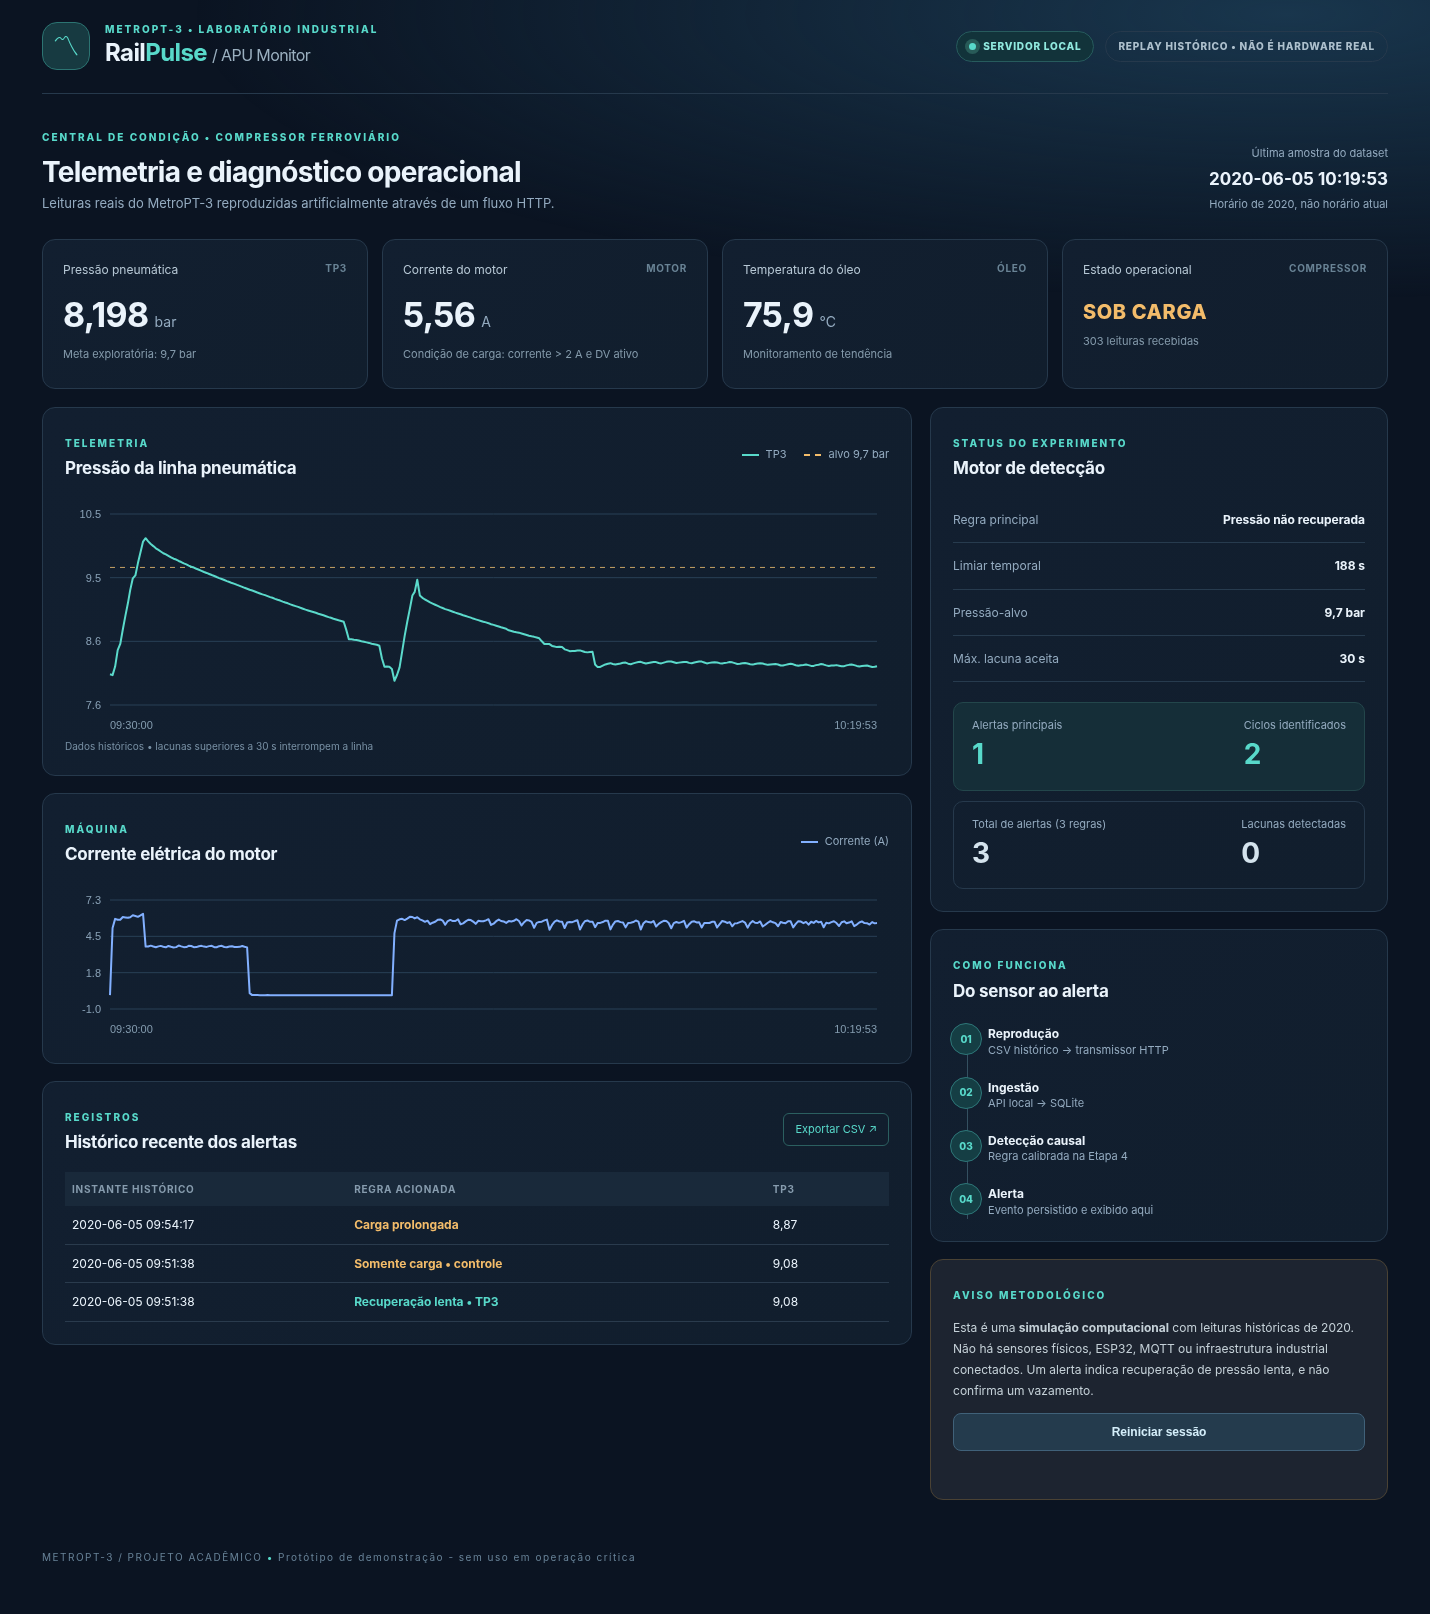
\includegraphics[width=0.75\columnwidth]{05_painel_railpulse.png}
\caption{Painel local RailPulse após replay de leituras históricas de F3; dados simulados no tempo de execução.}
\label{fig:painel}
\end{figure}

\section{Discussão}

\subsection{Significado físico e limitações do indicador}

A regra R1 combina estado elétrico-operacional com uma condição pneumática interpretável. Ela descarta fases que, apesar de longas, já haviam recuperado a pressão de referência. Essa interpretação é coerente com a física qualitativa de pressurização, mas a duração de recuperação não é identificador unívoco de vazamento, pois depende de consumo variável, pressão inicial e dinâmica do controle. A análise detalhada de F2 e F4 demonstra explicitamente que parte dos chamados pré-alertas resulta de ciclos que se recuperam normalmente, segundo a própria meta de pressão.

Os 20 avisos externos à proximidade dos eventos também não autorizam uma taxa de falsos positivos em sentido estrito. Para estimar esse indicador seriam necessários eventos de manutenção exaustivos, tempo de operação efetivamente observável e estados saudáveis auditados. Em vez disso, é defensável informar somente a carga operacional observada de avisos por calendário -- 5,94 avisos externos por 30 dias para R1 no intervalo de teste -- como uma razão descritiva dependente do recorte e das exclusões adotadas.

\subsection{Seleção de hipóteses e validade temporal}

A divisão calibração/teste impede usar diretamente registros posteriores para estimar os percentis; a equivalência de execução incremental verifica decisões sem consulta ao futuro. Essas propriedades não resolvem um tipo diferente de viés: o desenvolvimento das faixas de pressão, alvo e horizonte foi realizado após inspeção de eventos incluídos na avaliação final. Logo, os resultados são retrospectivos e informados pelo conjunto de avaliação. O P95--P99 foi calculado somente no período de calibração, mas a própria decisão de executar essa análise surgiu após a observação dos eventos.

Bergmeir, Hyndman e Koo~\cite{bergmeir2018note} estudam condições de validade da validação cruzada de séries autorregressivas; suas conclusões não implicam proibição geral da validação aleatória. Aqui, a divisão cronológica foi adotada pela natureza do fluxo de telemetria e para garantir disponibilidade temporal dos parâmetros, não como argumento de exclusividade estatística. Um estudo confirmatório exigirá parâmetros congelados antes de observar novas máquinas ou novos períodos.

\subsection{Avaliação das regras e utilidade prática}

O experimento não demonstra que R1 detecta mais eventos que R3: ambas apresentaram alertas antes dos três horários documentados. A contribuição comparativa disponível é redução de alertas quando a condição de pressão é incluída, sob elegibilidade inicial comum. A análise de sensibilidade mostra que aumentar seletividade via percentis mais altos implica descartar fases relativamente lentas; em um histórico com anotações incompletas, não se conhece a quantidade de defeitos não documentados eventualmente perdidos com essa escolha.

Para eventual adoção na manutenção, os alertas deveriam ser contextualizados por demanda pneumática, agrupamento de episódios, duração da permanência sob carga, estado da válvula, temperatura e inspeções físicas. Indicadores adicionais, como recuperação de pressão condicionada à demanda, poderiam fornecer especificidade maior, mas essa vantagem ainda não foi quantificada nesta pesquisa.

\subsection{Alcance da prova de conceito IoT}

A integração HTTP, SQLite e painel demonstra comunicação entre módulos de software e processamento incremental de dados históricos. Não demonstra disponibilidade embarcada, capacidade da rede celular, perda de pacotes, segurança cibernética, confiabilidade dos sensores ou adequação temporal à operação de um trem. Um estudo aplicado em campo exigiria hardware e canais reais, protocolos de autenticação, avaliação de falhas de comunicação, integração com procedimentos de manutenção e testes de segurança em Tecnologia Operacional (TO).

\subsection{Limitações e agenda de confirmação}

Os limites mais importantes são: (a) somente três eventos após a calibração; (b) rótulos extraídos de registros administrativos, com incerteza de início físico; (c) hipótese e parâmetros informados por inspeções exploratórias do teste; (d) cinco tempos censurados não tratados por técnicas de sobrevivência; (e) intervalos temporais irregulares e lacunas; (f) influência desconhecida do consumo pneumático; (g) uma única unidade instrumentalizada e uma única versão do dataset; e (h) replay local sem avaliação em ambiente de produção.

Para dar continuidade, recomenda-se pré-registrar uma configuração fixa, executar validação externa em outro período ou compressor, obter registros completos de manutenção e demanda, estudar análise de sobrevivência para tempo até recuperação com censura, expressar a carga de alarmes por horas válidas observadas, comparar regras com modelos estatísticos em protocolos equivalentes e avaliar instrumentação e rede reais. Sem isso, não se deve converter a proporção observada 3/3 em uma alegação de 100\% de sensibilidade.

\section{Conclusão}

Este estudo apresentou e revisou um detector interpretável de recuperação lenta de pressão em uma APU ferroviária usando 1.516.948 registros reais do MetroPT-3. O método identificou 10.417 ciclos completos elegíveis e, no teste cronológico retrospectivo, registrou 33 avisos sob a regra principal, contra 136 avisos de um critério puramente temporal com igual limiar. Treze avisos de R1 situaram-se nas duas horas anteriores aos registros de três eventos, enquanto outros 20 ocorreram fora das proximidades definidas para essas ocorrências.

A nova análise de sensibilidade confirma forte dependência da quantidade de avisos ao percentil de calibração: P95, P97,5 e P99 produziram, respectivamente, 363, 109 e 33 avisos. O protótipo de telemetria simulada reproduziu exatamente os 190 avisos das três regras originais, comprovando equivalência computacional no histórico analisado. O resultado sustenta o potencial do indicador como monitor de recuperação pneumática lenta para orientar inspeção; não demonstra previsão prospectiva confiável de vazamentos nem implantação IoT industrial física.

\section*{Declarações de transparência, disponibilidade e autoria}

DADOS: MetroPT-3 obtido do UCI Machine Learning Repository (DOI 10.24432/C5VW3R; licença CC BY 4.0). A reprodução exige baixar o CSV e conferir seu SHA-256, informado na Seção 3.1. SOFTWARE: os scripts da Etapa 4 e do protótipo da Etapa 5, tabelas, arquivos de parâmetros e o script complementar de sensibilidade são fornecidos em pacote de apoio. O código de análise adicional foi construído sobre o extrator da Etapa 4. ETICIDADE: não há participação de seres humanos nem identificação de passageiros nas variáveis examinadas. FINANCIAMENTO E CONFLITOS: devem ser confirmados pelo autor antes da submissão.

\appendices
\section{Rastreabilidade dos resultados}

\begin{table}[H]
\centering
\caption{Rastreabilidade dos resultados e artefatos.}
\label{tab:5}
\scriptsize
\setlength{\tabcolsep}{3pt}
\renewcommand{\arraystretch}{1.12}
\begin{tabularx}{\columnwidth}{@{}Y Y@{}}
\toprule
\textbf{Resultado documentado} & \textbf{Origem para reprodução} \\
\midrule
1.516.948 registros e SHA-256 & CSV original e parâmetros da Etapa 4 \\
15.769 fases; 10.417 ciclos & \texttt{ciclos\_carga.csv}; extrator da Etapa 4 \\
P99 = 188 s; carga = 337,12 s & \texttt{parametros.json}; calibração da Etapa 4 \\
R1 = 33; R2 = 21; R3 = 136 & \texttt{comparacao\_regras.csv}; \texttt{alertas\_ciclos.csv} \\
Horários de F2, F3 e F4 & \texttt{avaliacao\_falhas.csv} \\
190 correspondências exatas & \texttt{teste\_equivalencia.log}; \texttt{equivalencia.json} \\
P95 = 363; P97,5 = 109; P99 = 33 & \path{sensibilidade_temporal_exploratoria.csv}; script adicional \\
Figuras 1--3 e 5 & Arquivos originais das Etapas 4--6 \\
Figura 4 & \path{figura_sensibilidade_percentil.png} \\
\bottomrule
\end{tabularx}
\end{table}

\section{Recomendações para avaliação confirmatória}

O próximo experimento deve congelar os parâmetros da regra, registrar previamente o horizonte de avaliação e definir critérios de verdade-terreno antes de consultar dados inéditos. Devem ser obtidos, quando disponíveis, a demanda pneumática, os relatórios detalhados de reparo, estados operacionais certificados e duração efetiva do monitoramento. Só então será defensável estimar sensibilidade, precisão, taxa de alertas em condição saudável e intervalos de confiança.

\balance

\bibliographystyle{IEEEtran}

\bibliography{referencias}

\end{document}
